% Preprocessing pipeline — signal-processing paper style (monochrome, op-chain).
% raw frame -> MTCNN -> align -> crop+pad -> resize 256 -> normalise -> (branch) block-DCT.
% Compile:  pdflatex fig_2_preprocess_pipeline.tex
\documentclass[border=12pt]{standalone}
\usepackage{amsmath,amssymb}
\usepackage{tikz}
\usetikzlibrary{arrows.meta,calc,positioning}
\begin{document}
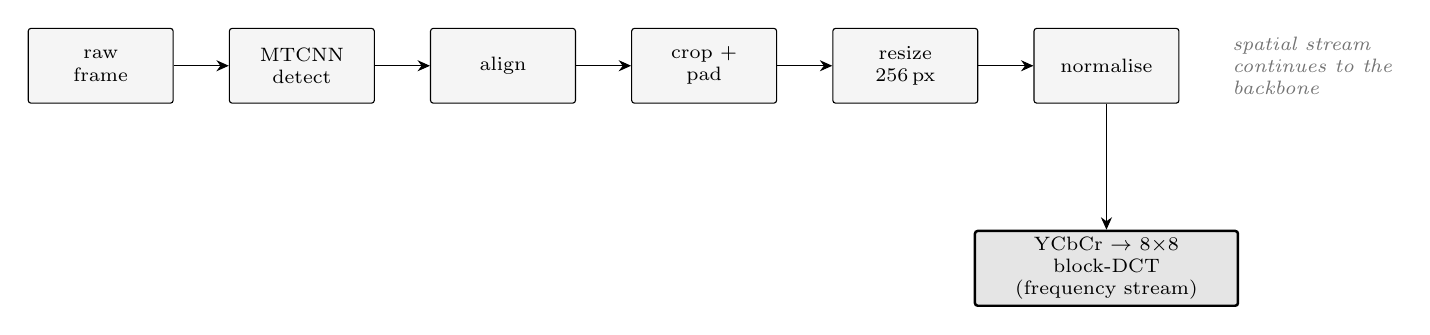
\begin{tikzpicture}[
  font=\small,
  node distance=0.7cm,
  box/.style={draw=black, thin, fill=black!4, rounded corners=1pt,
              text width=1.7cm, align=center, minimum height=0.95cm,
              inner sep=2pt, font=\scriptsize},
  freq/.style={draw=black, line width=0.9pt, fill=black!10, rounded corners=1pt,
               text width=3.2cm, align=center, minimum height=0.95cm,
               inner sep=2pt, font=\scriptsize},
  arr/.style={-{Stealth[length=4.5pt,width=4pt]}, thin},
  note/.style={font=\scriptsize\itshape, text=black!55, align=left},
]
% ---- spatial chain (left to right) ----
\node[box] (raw)                       {raw\\frame};
\node[box, right=of raw]   (mtcnn)     {MTCNN\\detect};
\node[box, right=of mtcnn] (align)     {align};
\node[box, right=of align] (crop)      {crop +\\pad};
\node[box, right=of crop]  (resize)    {resize\\256\,px};
\node[box, right=of resize] (norm)     {normalise};

\draw[arr] (raw)    -- (mtcnn);
\draw[arr] (mtcnn)  -- (align);
\draw[arr] (align)  -- (crop);
\draw[arr] (crop)   -- (resize);
\draw[arr] (resize) -- (norm);

% ---- spatial stream continues note ----
\node[note, right=0.55cm of norm] (cont) {spatial stream\\continues to the\\backbone};

% ---- frequency branch (down from normalise) ----
\node[freq, below=1.6cm of norm] (dct)
  {YCbCr $\rightarrow$ $8{\times}8$ block-DCT\\(frequency stream)};
\draw[arr] (norm.south) -- (dct.north);

\end{tikzpicture}
\end{document}
